\begin{textbox}{\href{https://compneuro.neuromatch.io/tutorials/W0D3_LinearAlgebra/student/W0D3_Tutorial1.html}{Linear Algebra (W0D3T1)} - Vectors}
\begin{subbox}{subbox}{A Vector}
\scriptsize
A vector, $\mathbf{v}$, is a short hand way of representing a list of numbers like $x$ and $y$ coordinates:
\begin{equation}
\mathbf{v} = 
\begin{bmatrix}
4 \\
1
\end{bmatrix},
\end{equation}

A 2-D vector $\mathbf{v}$ has a direction and a length. A normalized vector $\widetilde{\mathbf{v}}$ has a length 1.

\centering
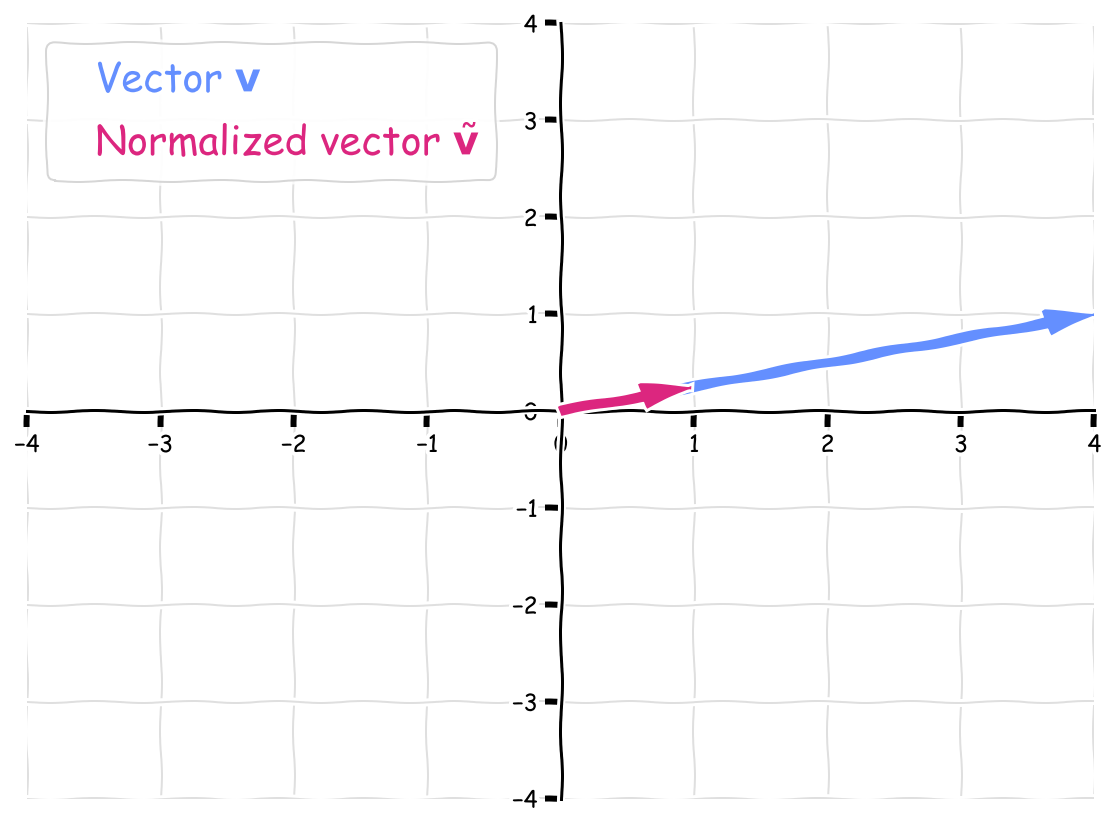
\includegraphics[scale=0.1]{Figures/PreCourse/Figure1.png}
\end{subbox}

\begin{subbox}{subbox}{Linear Combination of Vectors}
\scriptsize
Two vectors $\mathbf{x}$ and $\mathbf{y}$ can be added together and multiplied by parameters $a$ and $b$ to get a new vector $\mathbf{z}$
\begin{equation}
\mathbf{z} = a\mathbf{x} + b\mathbf{y}
\end{equation}

given $\mathbf{x} = \begin{bmatrix}3 \\ 1 \end{bmatrix}$ and $\mathbf{y} = \begin{bmatrix}-1 \\ 2 \end{bmatrix}$, and $a=-1$ and $b=2$
\begin{equation*}
\begin{bmatrix}-6 \\ 3 \end{bmatrix}= -1\begin{bmatrix}3 \\ 1 \end{bmatrix} +2 \begin{bmatrix}-1 \\ 2 \end{bmatrix}.
\end{equation*}
\centering
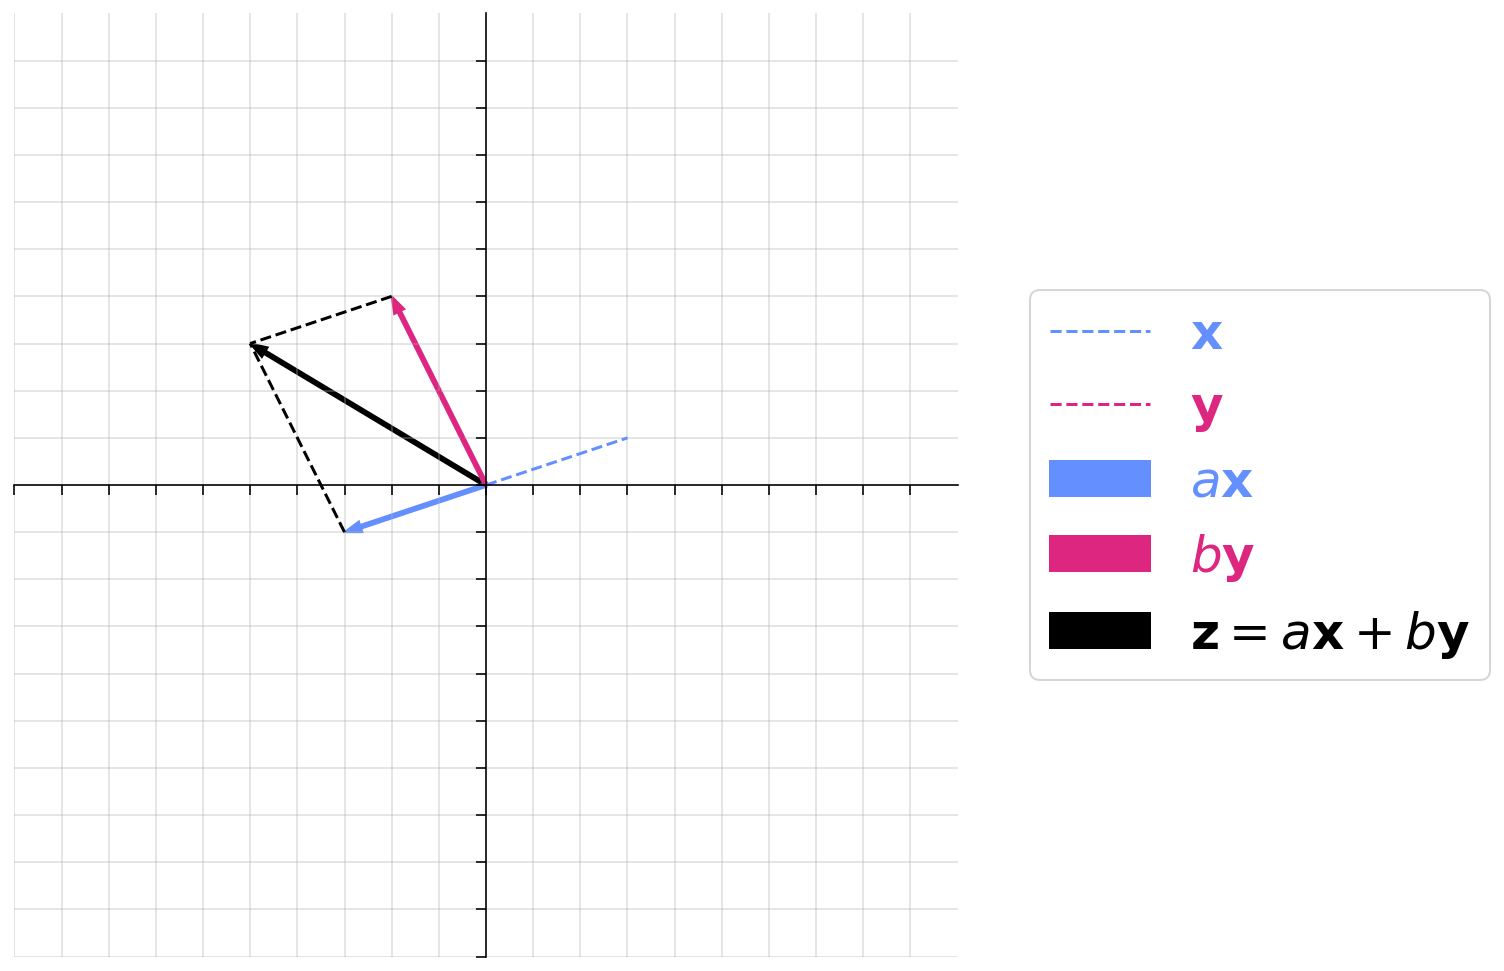
\includegraphics[scale=0.15]{Figures/PreCourse/Figure3.png}
\end{subbox}
\begin{subbox}{subbox}{The Geometry of the Dot Product $\mathbf{w}\cdot\mathbf{r}$}
\scriptsize
An alternate way of defining the dot product is as the multiple of the lengths of the two vectors and the angle between them $\theta$:

\begin{equation}
\mathbf{x} \cdot \mathbf{y} = ||\mathbf{x}|| \cdot ||\mathbf{y}|| \cdot \cos(\theta).
\end{equation}

\end{subbox}
\end{textbox}
%%%%%%%%%%%%%%%%%%%%%%%%%%%%%%%%%%%%%%%%%%%%%%%%%%
\begin{textbox}{Linear Algebra (W0D3T1) - Vectors}
\begin{subbox}{subbox}{Dot Product $\mathbf{w}\cdot\mathbf{r}$}
\scriptsize
Given two retinal neurons with varying firing rates ($r_1$ and $r_2$).  The retinal firing rates can be represented as the vector $\mathbf{r} = \begin{bmatrix} r_1\\ r_2\\ \end{bmatrix}$.

The weights from each of these to an LGN neuron. The weights are represented with the vector $\mathbf{w} = \begin{bmatrix} w_1\\ w_2\\ \end{bmatrix}$.

The LGN firing rate is the dot product of the retinal firing rate vector and the weight vector:
\begin{equation}
g = \mathbf{w}\cdot\mathbf{r} = w_1r_1 + w_2r_2
\end{equation}

\centering
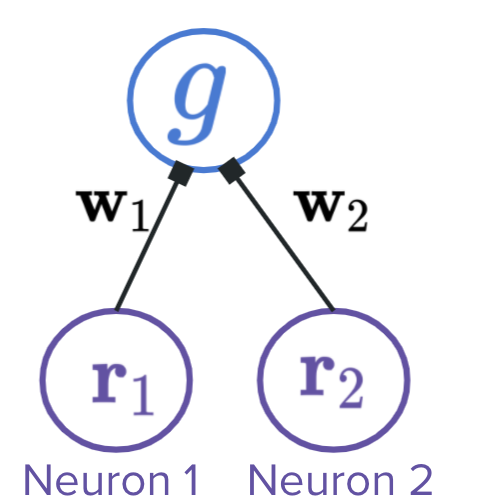
\includegraphics[scale=0.3]{Figures/PreCourse/Figure2.png}
\end{subbox}

\end{textbox}
%%%%%%%%%%%%%%%%%%%%%%%%% 
%%%%%%%%%%%%%%%%%%%%%%%%%
\begin{textbox}{Linear Algebra (W0D3T2) - Matrices}
\begin{subbox}{subbox}{Intro to Matrices}
\scriptsize
We will look at a group of 2 LGN neurons which get input from 2 retinal neurons: we will call the population of LGN neurons population $p$. Below, we have the system of linear equations that dictates the neuron models for each population. $r_1$ and $r_2$ correspond to the retinal neural activities (of neuron 1 and 2). $g_{p_1}$ and  $g_{p_2}$ correspond to the responses of the LGN neurons 1 and 2 in population $p$. 

\begin{align}
r_1 + 3r_2 &= g_{p_1} \\
2r_1 + r_2 &= g_{p_2} 
\end{align}
Cast each equation (i.e., $g_{p_1}$ and $g_{p_2}$) as a matrix-vector multiplication: 

\begin{equation}
\mathbf{g}_p = \mathbf{P}\mathbf{r}
\end{equation}

where \begin{equation}\mathbf{P}=
\begin{bmatrix}
1 & 3 \\
2 & 1
\end{bmatrix}
\end{equation}

is the weight matrix to population $p$. 
\end{subbox}
\end{textbox}
\begin{textbox}{Linear Algebra (W0D3T2) - Matrices}

\begin{subbox}{subbox}{Matrices as Linear Transformations}
\scriptsize
Matrices can be thought of as enacting linear transformations. When multiplied with a vector, they transform it into another vector. In fact, they are transforming a grid of space in a linear manner: the origin stays in place and grid lines remain straight, parallel, and evenly spaced.

\centering
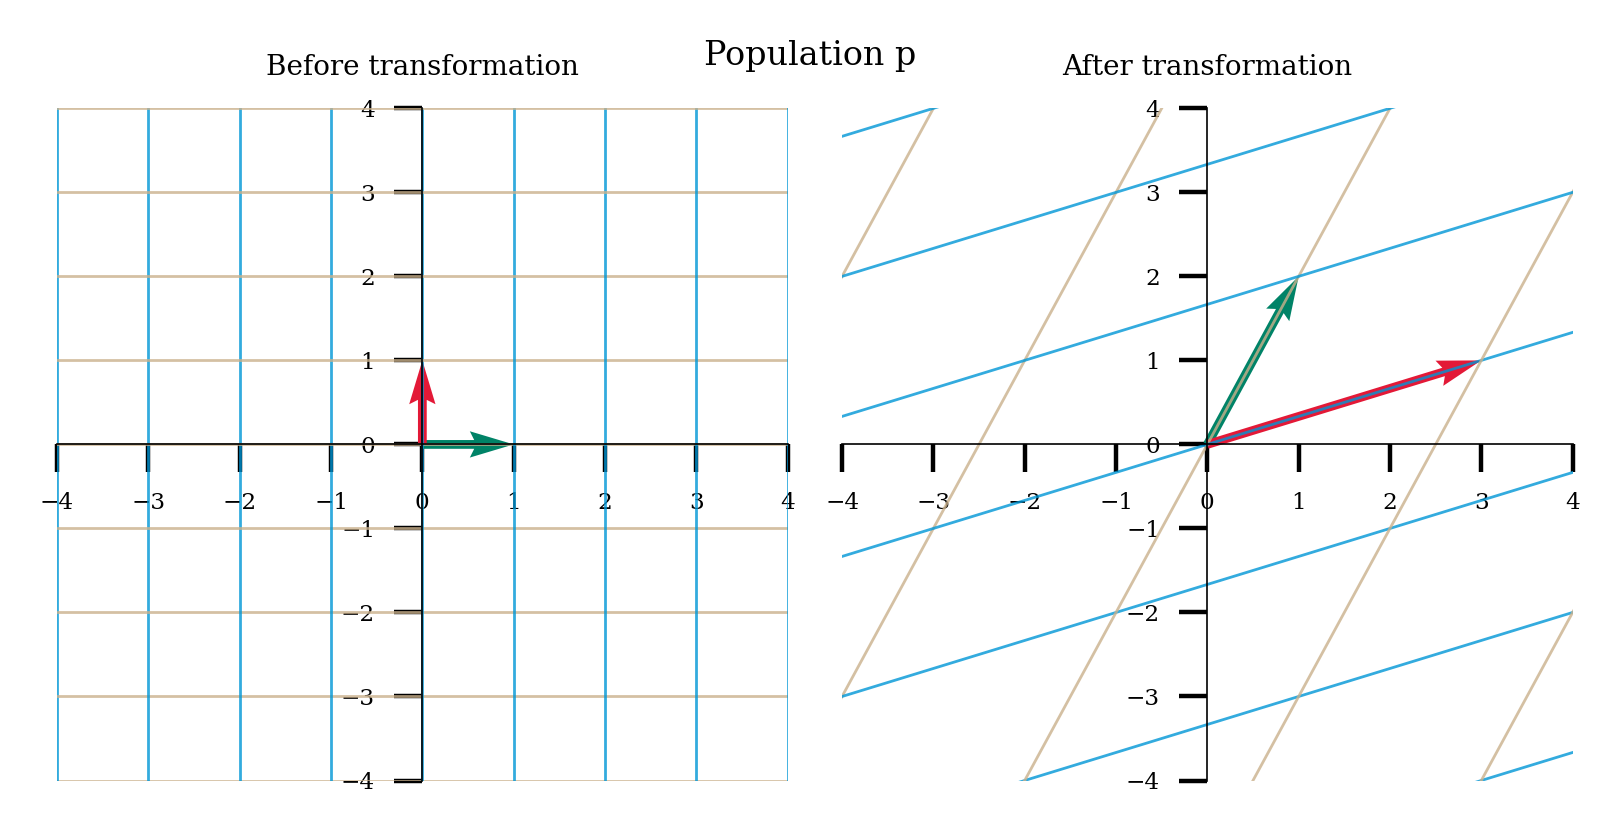
\includegraphics[scale=0.5]{Figures/PreCourse/Figure4.png}
\end{subbox}


\begin{subbox}{subbox}{Eigenvalues \& Eigenvectors}
\tiny
Eigenvectors, $\mathbf{v}$ of a matrix $\mathbf{W}$ are vectors that, when multipled by the matrix, equal a scalar multiple of themselves. That scalar multiple is the corresponding eigenvalue, $\lambda$.

\begin{equation}
\mathbf{W}\mathbf{v} = \lambda\mathbf{v}
\end{equation}

If we have one eigenvector for a matrix, we technically have an infinite amount: every vector along the span of that eigenvector is also an eigenvector. So, we often use the unit vector in that direction to summarize all the eigenvectors along that line. 

Just by looking at eigenvectors before and after a transformation, can you describe what the transformation is in words? Try for each of the two plots below.

\centering
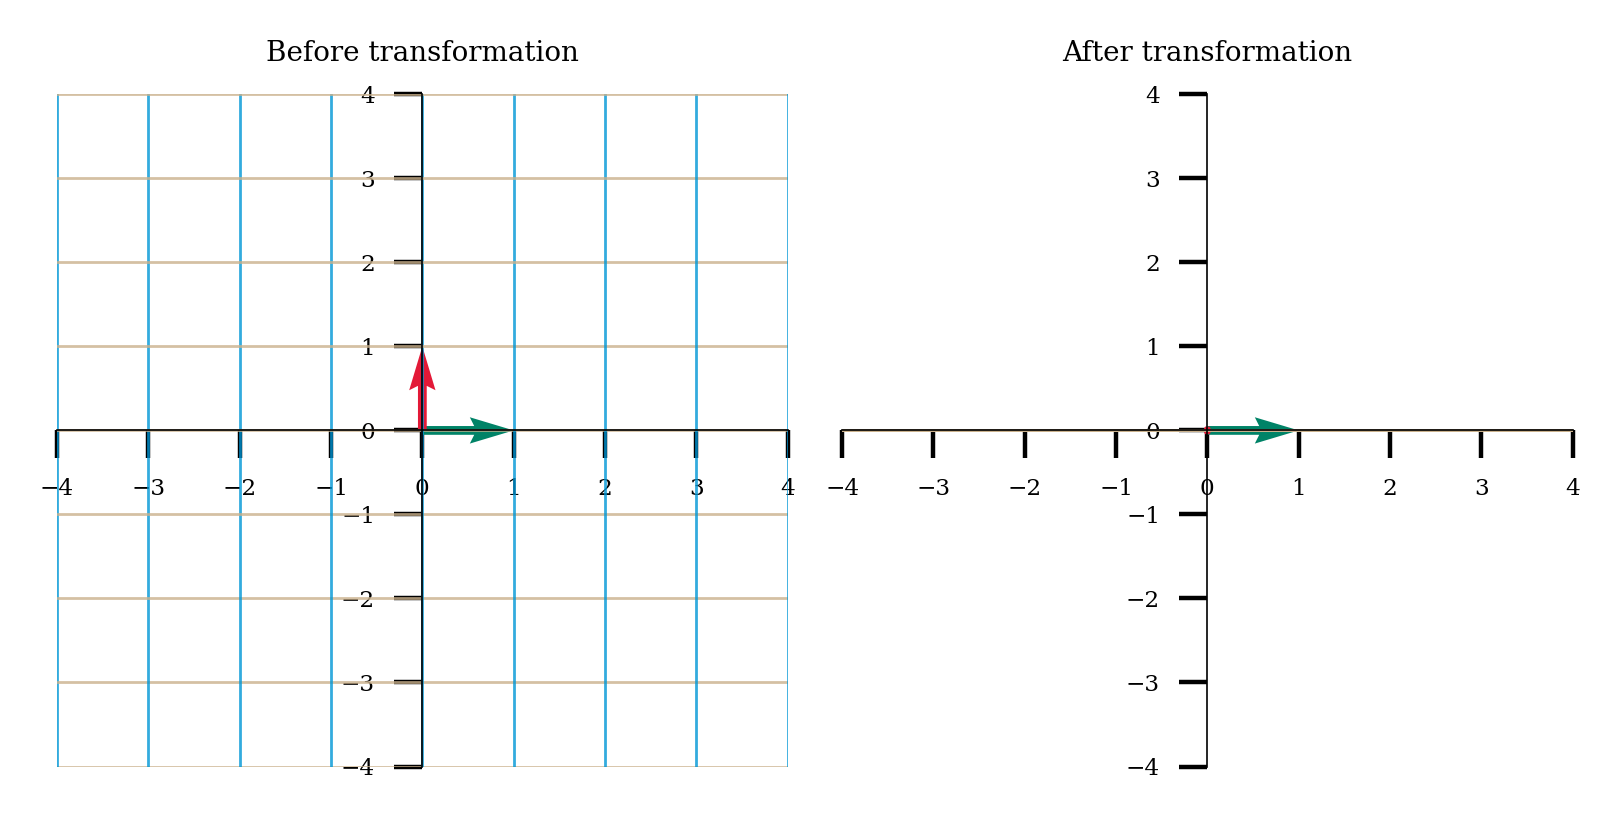
\includegraphics[scale=0.1]{Figures/PreCourse/Figure5.png}

\end{subbox}

\begin{subbox}{subbox}{Matrix Multiplication}
\tiny
We sometimes want to multiple two matrices together, instead of a matrix with a vector. Let's say we're multiplying matrices $\mathbf{A}$ and $\mathbf{B}$ to get $\mathbf{C}$:
\begin{equation}
\mathbf{C} = \mathbf{A}\mathbf{B}\text{.}
\end{equation}

We take the dot product of each row of A with each column of B. The resulting scalar is placed in the element of $\mathbf{C}$ that is the same row (as the row in A) and column (as the column in B). So the element of $\mathbf{C}$ at row 4 and column 2 is the dot product of the 4th row of $\mathbf{A}$ and the 2nd column of $\mathbf{B}$. We can write this in a formula as:
\begin{equation}\mathbf{C}_{\text{row i, column j}} = \mathbf{A}_{\text{row i}} \cdot \mathbf{B}_{\text{column j}}
\end{equation}
\end{subbox}
\end{textbox}
